\documentclass[10pt,landscape]{article}
\usepackage{multicol}
\usepackage[landscape]{geometry}
\usepackage[procnames]{listings}
\usepackage[parfill]{parskip}
\usepackage{fixltx2e}
\usepackage[T1]{fontenc}
\usepackage{lmodern}
\usepackage{graphicx}

% "define" Scala
\usepackage[T1]{fontenc}  
\usepackage[scaled=0.82]{beramono}  
\usepackage{microtype} 

\sbox0{\small\ttfamily A}
\edef\mybasewidth{\the\wd0 }

\lstdefinelanguage{scala}{
  morekeywords={abstract,case,catch,class,def,%
    do,else,extends,false,final,finally,%
    for,if,implicit,import,match,mixin,%
    new,null,object,override,package,%
    private,protected,requires,return,sealed,%
    super,this,throw,trait,true,try,%
    type,val,var,while,with,yield},
  sensitive=true,
  morecomment=[l]{//},
  morecomment=[n]{/*}{*/},
  morestring=[b]",
  morestring=[b]',
  morestring=[b]"""
}

\usepackage{color}
\definecolor{dkgreen}{rgb}{0,0.6,0}
\definecolor{gray}{rgb}{0.5,0.5,0.5}
\definecolor{mauve}{rgb}{0.58,0,0.82}

% Default settings for code listings
\lstset{frame=tb,
  language=scala,
  aboveskip=3mm,
  belowskip=3mm,
  showstringspaces=false,
  columns=fixed, % basewidth=\mybasewidth,
  basicstyle={\small\ttfamily},
  numbers=none,
  numberstyle=\footnotesize\color{gray},
  % identifierstyle=\color{red},
  keywordstyle=\color{blue},
  commentstyle=\color{dkgreen},
  stringstyle=\color{mauve},
  frame=single,
  breaklines=true,
  breakatwhitespace=true,
  procnamekeys={def, val, var, class, trait, object, extends},
  procnamestyle=\ttfamily\color{red},
  tabsize=2
}

\lstnewenvironment{scala}
{\lstset{language=scala}}
{}
\lstnewenvironment{cpp}
{\lstset{language=C++}}
{}
\lstnewenvironment{bash}
{\lstset{language=bash}}
{}
\lstnewenvironment{verilog}
{\lstset{language=verilog}}
{}



% Remove section numbering
\setcounter{secnumdepth}{0}

\geometry{top=.75cm,left=.75cm,right=.75cm,bottom=.75cm}


\pagestyle{empty}
\setlength{\parskip}{0cm}

\makeatletter
\renewcommand{\section}{\@startsection{section}{1}{0mm}%
                                {-0.5ex plus 4ex}%
                                {-0.01ex plus .01ex}%x
                                {\normalfont\large\bfseries}}
\renewcommand{\subsection}{\@startsection{subsection}{2}{0mm}%
                                {-0.5ex plus 4ex}%
                                {-0.01ex plus .01ex}%
                                {\normalfont\normalsize\bfseries}}
\renewcommand{\subsubsection}{\@startsection{subsubsection}{3}{0mm}%
                                {-0.01ex plus 0.01ex}%
                                {-0.01ex plus .01ex}%
                                {\normalfont\small\bfseries}}
\makeatother

\begin{document}
\begin{multicols}{3}

\newcommand*\ruleline[1]{\par\noindent\raisebox{.8ex}{\makebox[\linewidth]{\hrulefill\hspace{1ex}\raisebox{-.8ex}{#1}\hspace{1ex}\hrulefill}}}
\renewcommand{\tabcolsep}{.5mm}

\ruleline{\Large{\textbf{Chisel3 Testing Cheat Sheet}}}
\begin{center}
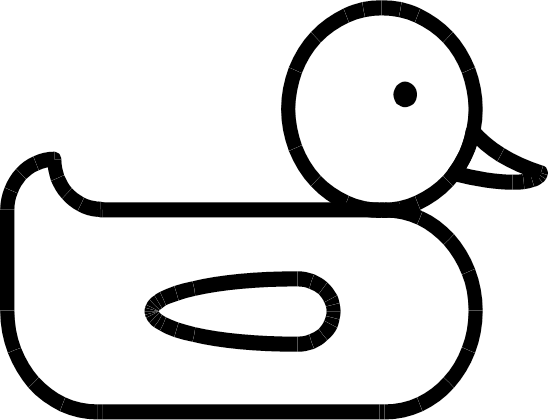
\includegraphics[scale=0.02]{bigduck.png} Version 0.5 (beta): \today
\end{center}

\fbox{ \parbox{0.95\columnwidth} {
\subsection{Notation In This Document}:
\subsubsection{For Functions and Constructors}: \newline
Arguments given as \texttt{kwd:type} (name and type(s)) \newline
Arguments in brackets (\texttt{[...]}) are optional.
\subsubsection{For Operators}: \newline
\texttt{c}, \texttt{x}, \texttt{y} are Chisel \texttt{Data};
\texttt{n}, \texttt{m} are Scala \texttt{Int} \newline
\texttt{w(x)}, \texttt{w(y)} are the widths of \texttt{x}, \texttt{y} (respectively) \newline
\texttt{minVal(x)}, \texttt{maxVal(x)} are the minimum or \newline
\phantom{x} maximum possible values of \texttt{x}
} }

\section{Testing } \hrulefill
\subsection
Chisel provides a evolving family of testers with different capabilities. A tester typically is invoked
from scalatest. For example:
\begin{scala}
class CounterSpec extends ChiselPropSpec {
  property("Counter should wrap") {
    assertTesterPasses {
        new WrapTester(42)
      }
    }
  }
\end{scala}
\subsection{BasicTester}: \newline
\verb$BasicTester$: supports creation of a circuit and provides simple chisel operations and
a family of assert statements.
\begin{scala}
class WrapTester(max: Int)
  extends BasicTester {
  val (cnt,wrap) = Counter(Bool(true),max)
  when(wrap) {
    assert(cnt === UInt(max - 1))
    stop()
  }
}
\end{scala}
\subsection{Chisel-Testers}: \newline
Additional testers can be found in the ucb-arg/chisel-testers repository. Current Testers are: \newline
\subsection{StandardTester}: \newline
\verb$Standard Tester$: is a class with functions for testing \verb$Module$s, connecting and communicating with a simulator: \newline
\begin{tabular*}{\columnwidth}{@{\extracolsep{\fill} } l l}
\verb$reset([n:Int])$ & reset the DUT for \verb$n$ (default 1) clocks \\
\verb$step(n:Int$) & steps the DUT for \verb$n$ clocks \\
\hline \end{tabular*} \begin{tabular*}{\columnwidth}{@{\extracolsep{\fill} } l l l}
\verb$poke(data:Bits, x:BigInt)$ & writes \verb$x$ to wire \verb$data$ \\
\multicolumn{2}{l}{\texttt{poke(data:Aggregate, x:Array[BigInt])}} \\
\multicolumn{2}{l}{\phantom{x} writes values from \texttt{x} to corresponding wires in \texttt{data}} \\
\verb$peek(data:Bits): BigInt$ & reads from wire \verb$data$ \\
\multicolumn{2}{l}{\texttt{peek(data:Aggregate): Array[BigInt]}} \\
\multicolumn{2}{l}{\phantom{x} reads multiple values from source wires in \texttt{data}} \\
\hline \end{tabular*} \begin{tabular*}{\columnwidth}{@{\extracolsep{\fill} } l l l}
\multicolumn{2}{l}{\texttt{expect(good:Boolean, msg:String): Boolean}} \\
\multicolumn{2}{l}{\phantom{x} fails unless \texttt{good} is \texttt{True}, \texttt{msg} should describe the test} \\
\multicolumn{2}{l}{\texttt{expect(data:Bits, target:BigInt): Boolean}} \\
\multicolumn{2}{l}{\phantom{x} fails unless the value in wire \texttt{data} equals \texttt{target}} \\
\end{tabular*}
\subsection{Defining}: \newline
Subclass \verb$Tester$ with testing code:
\begin{scala}
class MuxTester(c:Mux) extends Tester(c) {
  for (sel <- 0 until 2) {
    poke(c.io.sel, sel)
    poke(c.io.in0, 0); poke(c.io.in1, 1)
    step(1)
    expect(c.io.out, sel)
  }
}
\end{scala}
\subsection{Hardware IO Testers}: \newline
The Hardware IO Testers run all tests by implementing small FSM's and vectors of input and output
values.  In general hardware testers are faster than the standard tester. There currrently two forms
\subsection{Stepped Tester}: \newline
\verb$SteppedHWIOTester$: works like the Standard Tester but does not support the peek command
\subsection{Defining}: \newline
Subclass \verb$SteppedHWIOTester$ with testing code:
\begin{scala}
class AdderTests extends SteppedHWIOTester {
  val dut = Module( new Adder(10) )
  rnd.setSeed(0L)
  for (i <- 0 until 10) {
    val in0 = rnd.nextInt(1 << dut.w)
    val in1 = rnd.nextInt(1 << dut.w)
    poke(dut.io.in0, in0)
    poke(dut.io.in1, in1)
    expect(dut.io.out, (in0 + in1) & ((1 << dut.w) - 1))

    step(1)
  }
}
\end{scala}
\subsection{Decoupled Tester}: \newline
\verb$OrderedDecoupledHWIOTester$: tests Modules with IO implementing \verb$DeqIO$, \verb$EnqIO$,
\verb$Valid$ or \verb$Decoupled$ interfaces, automatically handling the ready/valid protocol.
\subsection{Defining}: \newline
Subclass \verb$OrderedDecoupledHWIOTester$ with testing code:
\begin{scala}
class DecoupledRealGCDTests4 extends OrderedDecoupledHWIOTester {
  val dut = Module(new RealGCD())
  for {
    i <- 1 to 10
    j <- 1 to 10
  } {
    val gcd_value = computeGcdResults(i, j)

    inputEvent(dut.io.in.bits.a -> i,
               dut.io.in.bits.b -> j)
    outputEvent(dut.io.out.bits -> gcd_value)
  }
}
\end{scala}

\end{multicols}
\end{document}
